\documentclass{article}
\usepackage[margin=1.5cm,bottom=2cm]{geometry}
\usepackage{fancyhdr}
\usepackage{graphicx}
\pagestyle{fancy}
\usepackage{amsmath}

\begin{document}
%\fancyhead[L]{ 
\includegraphics[width=2cm]{/Users/tjwilli/google_drive/course_materials/global/au_logo.png} }
\fancyhead[R]{PHYS 2250: General Physics II}
\fancyfoot[C]{\thepage}
\vspace*{0cm}
\begin{center}
	{\LARGE \textbf{Quiz 5}}\\
	\vspace{0.25cm}
	%{\Large Vector Review (Ungraded)}\\
	\vspace{0.25cm}
%	{\Large Friday, September 17}
\end{center}
The following information may or may not be of use:\\
\hrulefill\\
\begin{align*}
	\text{Electron current:}\ i&=nA\overline{v}\\
	\text{Conventional current:}\ I&=\left|q\right|i\\
	\text{Bio-Savart:}\ 
	\Delta \vec{B}&=\frac{\mu_0}{4\pi}\frac{I\Delta\vec{l}\times \hat{r}}{r^2}\\
	\text{Straight Wire:}\ \left|\vec{B}\right|&=\frac{\mu_0}{4\pi}\frac{LI}{r\sqrt{r^2+\left(L/2\right)^2}}\\
	\text{Very long straight wire:}\ \left|\vec{B}\right|&\approx \frac{\mu_0}{4\pi}\frac{2I}{r}\\
	\text{Center of loop of current: }\ \left|\vec{B}\right|&=\frac{\mu_0}{4\pi}\frac{2\pi R^2I}{\left(z^2+R^2\right)^{3/2}}
\end{align*}

\hrulefill \\
\\
A very long wire carrying a current $I$ is kinked in the middle so that it forms a small loop of radius $R$. What is the magnetic field (both magnitude and direction) at the center of the loop? Express your answer in terms of $\mu_0$, $I$, and $R$. Use a coordinate system where $+x$ points to the right ($\rightarrow$) and $+y$ points up ($\uparrow$).
\begin{center}
	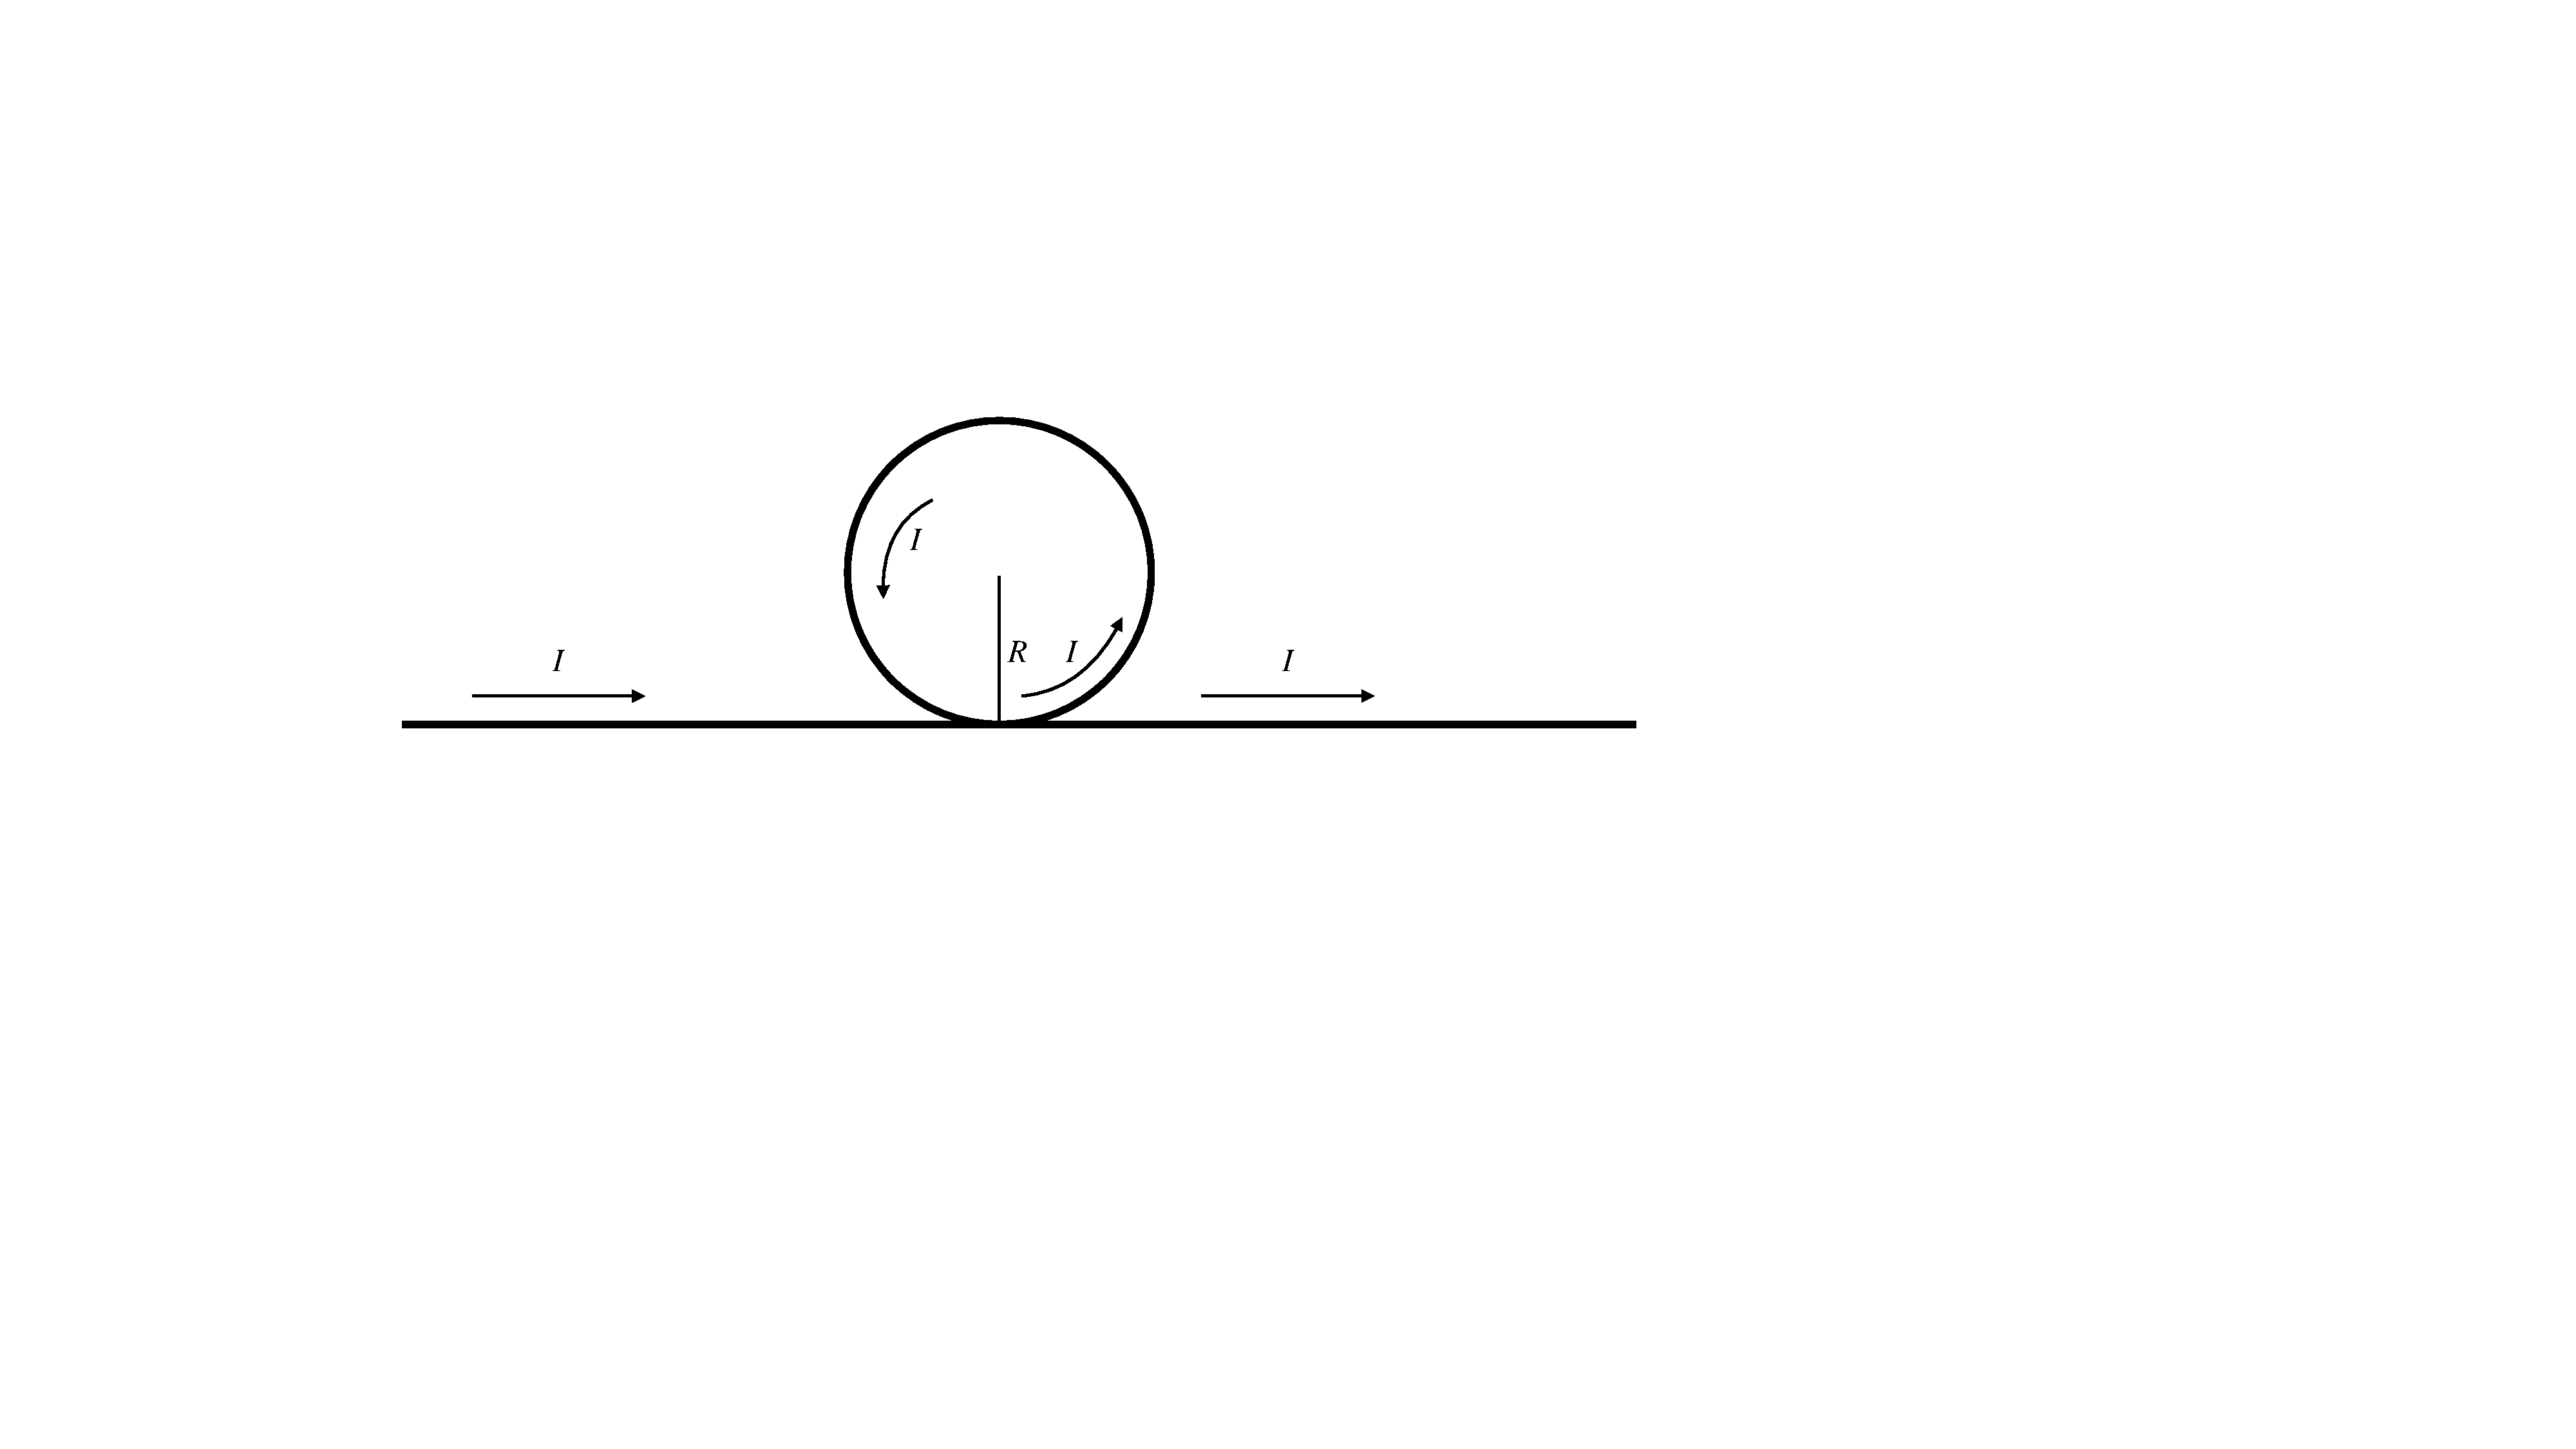
\includegraphics[width=.75\textwidth]{quiz_img}
\end{center}

\section*{Solution}
\begin{math}
	\vec{B} = \vec{B}_\mathrm{long\ wire} + \vec{B}_\mathrm{loop}\\\\
	\left|\vec{B}_\mathrm{long\ wire}\right|\approx \frac{\mu_0}{4\pi}\frac{2I}{r}\\\\
	r=R\implies 	\left|\vec{B}_\mathrm{long\ wire}\right|\approx \frac{\mu_0}{4\pi}\frac{2I}{R}\\\\
	\text{Right hand rule: }\hat{B}_\mathrm{long\ wire} = \hat{z}\\\\
	\vec{B}_\mathrm{long\ wire}\approx \frac{\mu_0}{4\pi}\frac{2I}{R}\hat{z}\\\\\\
	\left|\vec{B}_\mathrm{loop}\right|=\frac{\mu_0}{4\pi}\frac{2\pi R^2I}{\left(z^2+R^2\right)^{3/2}}\\\\
	z=0\implies \left|\vec{B}_\mathrm{loop}\right|=\frac{\mu_0}{4\pi}\frac{2\pi R^2I}{\left(R^2\right)^{3/2}}=\frac{\mu_0}{4\pi}\frac{2\pi I}{R}\\\\
	\text{Right hand rule: }\hat{B}_\mathrm{loop} = \hat{z}\\\\
	\vec{B}_\mathrm{loop}=\frac{\mu_0}{4\pi}\frac{2\pi I}{R} \hat{z}\\\\
	\vec{B} = \vec{B}_\mathrm{long\ wire} + \vec{B}_\mathrm{loop}=\frac{\mu_0}{4\pi}\frac{2I}{R}\hat{z}+\frac{\mu_0}{4\pi}\frac{2\pi I}{R} \hat{z}=\frac{\mu_0}{4\pi}\frac{2I}{R}\left(1+\pi \right)\hat{z}\\\\
	\vec{B}=\frac{\mu_0}{4\pi}\frac{2I}{R}\left(1+\pi \right)\hat{z}
\end{math}
\end{document}